\documentclass[12pt,a4paper,oneside]{book} 
\usepackage[utf8]{inputenc}
\usepackage[spanish]{babel}
\usepackage{amsmath}
\usepackage{amsfonts}
\usepackage{amssymb}
\usepackage{abstract} % Allows abstract customization
\renewcommand{\abstractnamefont}{\normalfont\bfseries} % Set the "Abstract" text to bold
\renewcommand{\abstracttextfont}{\normalfont\small\itshape} % Set the abstract itself to small italic text


\usepackage{amssymb, amsmath}
\usepackage{graphicx}
\usepackage[left=2.54cm,right=2.54cm,top=2.54cm,bottom=2.54cm]{geometry}

\begin{document}
	
	\thispagestyle{empty} 
	
	\begin{center} 
		\LARGE{UNIVERSIDAD PRIVADA DE TACNA} \\[0.5cm] 
		\Large{FACULTAD DE INGENIERÍA DE SISTEMAS}\\[0.5cm] 
		\large{ ESCUELA PROFESIONAL DE INGENIERÍA SISTEMAS} 
	\end{center}
	
	\begin{figure}[htb]
		\centering 
\includegraphics[width=6cm, height=7cm]{img/uptlogo.jpg}
	\end{figure}
	
	\begin{center} 
			\LARGE{\bf TRABAJO ENCARGADO \newline DATOS NO ESTRUCTURADOS \newline UNIDAD III }\\ \vspace{.25cm}
		
	\end{center}

	\begin{center} 
		
		\textbf {CURSO}\\ 
		\large Base de Datos II \\
		
		\textbf {DOCENTE}\\
		\large Mag. Patrick Cuadros Quiroga\\
	
		\textbf {INTEGRANTES}\\
		\large Tarqui Montalico, Risther Jaime - 2017057857 \\
		\large Limache Victorio, V\'ictor Piero - 2017057857 \\
		\large S\'anchez Rodr\'iguez, Bayron - 2017057857 \\
		\large Liendo Velasquez, Joaqu\'in - 2017057857 \\
		\large Callata Flores, Rafael - 2017057857 \\
		
	\end{center}

	
	
	\begin{center} 
		\Large \textsc{Tacna - Perú} \\
		\Large \textsc{2020 } 
	\end{center}

	\newpage
	
	%%INICIO abstract
	\begin{abstract}

		En este articulo se muestra la importancia de los Datos no Estructurados, dando las definiciones necesarias, también se muestra 3 formas en las cuales se pueden extraer Datos no estructurados, algunas aplicaciones conocidas que se le dan y se finaliza con un ejemplo no practico con una red social conocida. \\
		\begin{center}
			
			\textbf{Abstract}
		\end{center}
		This article shows the importance of Unstructured Data, giving the necessary definitions, it also shows 3 ways in which unstructured Data can be extracted, some known applications that are given and ends with an impractical example with a known social network. \\
	\end{abstract}
	%%FIN abstract
	
	\newpage
	
	\begin{center} 
		\LARGE{\bf DATOS NO ESTRUCTURADOS \newline UNIDAD III }\\ \vspace{.25cm}
	\end{center}

	
	\begin{enumerate}
		
		\item \textbf{Introducci\'on.} \\
		
				Antes de hablar sobre datos no estructurados, debe comprender qué son los datos estructurados. Cuando hablamos de datos estructurados nos referimos a la información que habitualmente se encuentra en la mayoría de bases de datos. Son archivos de tipo texto que generalmente se muestran en filas y columnas con títulos. Son datos que todas las herramientas de minería de datos pueden ordenar y procesar fácilmente. Podríamos verlo como si se tratara de un archivador perfectamente organizado donde todo está identificado, etiquetado y de fácil acceso.\\
		
		
		\item \textbf{Objetivo.}
		
				Mostrar en este artículo que existe todo una serie de datos "no tradicionales"(imágenes, audio, texto, etc.) que pueden ser analizados y de los que cuales se puede extraer valor. \\
				
				
		\item \textbf{Autores.}
		
				\begin{itemize}
					
					\item	Limache Victorio, V\'ictor Piero 
					\item	Tarqui Montalico, Risther Jaime 
					\item	S\'anchez Rodr\'iguez, Bayron 
					\item	Liendo Velasquez, Joaqu\'in 
					\item	Callata Flores, Rafael 
					
				\end{itemize}
			
		\item \textbf{Desarrollo.}
				\begin{enumerate}
					\item \textbf{¿QUÉ SON LOS DATOS NO ESTRUCTURADOS?.} \\
					
					En su definición más básica, simplemente significa cualquier forma de datos que no encaja fácilmente en un modelo relacional o un conjunto de tablas de base de datos desestructurado.\\
					
					Los datos no estructurados, generalmente son datos binarios que no tienen estructura interna identificable. Es un conglomerado masivo y desorganizado de varios objetos que no tienen valor hasta que se identifican y almacenan de manera organizada.\\
					
					Una vez que se organizan, los elementos que conforman su contenido pueden ser buscados y categorizados (al menos hasta cierto punto) para obtener información.\\
					
					Aunque parezca increíble, la base de datos con información estructurada de una empresa, ni siquiera contiene la mitad de la información que hay disponible en la empresa lista para ser usada. El 80\% de la información relevante para un negocio se origina en forma no estructurada, principalmente en formato texto.\\
					
					
					\item \textbf{TIPOS DE DATOS NO-ESTRUCTURADOS:}
					
					Entre los distintos tipos de datos no estructurados tenemos:
					
					\begin{enumerate}
						
						\item Correos electrónicos
						
						\item Archivos de procesador de texto como Word
						
						\item Archivos PDF
						
						\item Hojas de cálculo como Excel.
						
						\item Imágenes digitales como 
						formatos bmp, tiff
						
						\item Vídeo como mp4, avi
						
						\item Audio como mp3
						
						\item Publicaciones en redes sociales.
						
						\item Presentaciones como PowerPoint
						
						
					\end{enumerate}
					
					Mirando esa lista, te podrías preguntar qué tienen en común estos archivos. Se trata de archivos que pueden ser almacenados y administrados sin que el sistema tenga necesidad de entender el formato del archivo. Al no estar organizado el contenido de estos archivos, estos datos suelen ser almacenados en carpetas locales en las redes de las empresas o en la nube como Dropbox, Google drive o SharePoint.\\
					
					\item \textbf{FORMAS DE EXTRACCIÓN DE DATOS NO ESTRUCTURADOS:}
					
					Entre los métodos de extracción de datos no estructurados tenemos:\\
					
					\begin{enumerate}
						
						\item \textbf{ Web Scraping (Rascado de datos)}
							Se podría definir como la técnica por la que un equipo de desarrolladores es capaz de rascar, escrapear o liberar datos de páginas web de gobiernos, instituciones públicas u organizaciones para acceder a datos privados o públicos que puedan ser publicados o distribuidos en formato abierto. El problema es que la mayoría de los datos de interés están en formatos no reutilizables y poco transparentes como un PDF, por ejemplo.
							
							\begin{figure}[htb]
								\centering 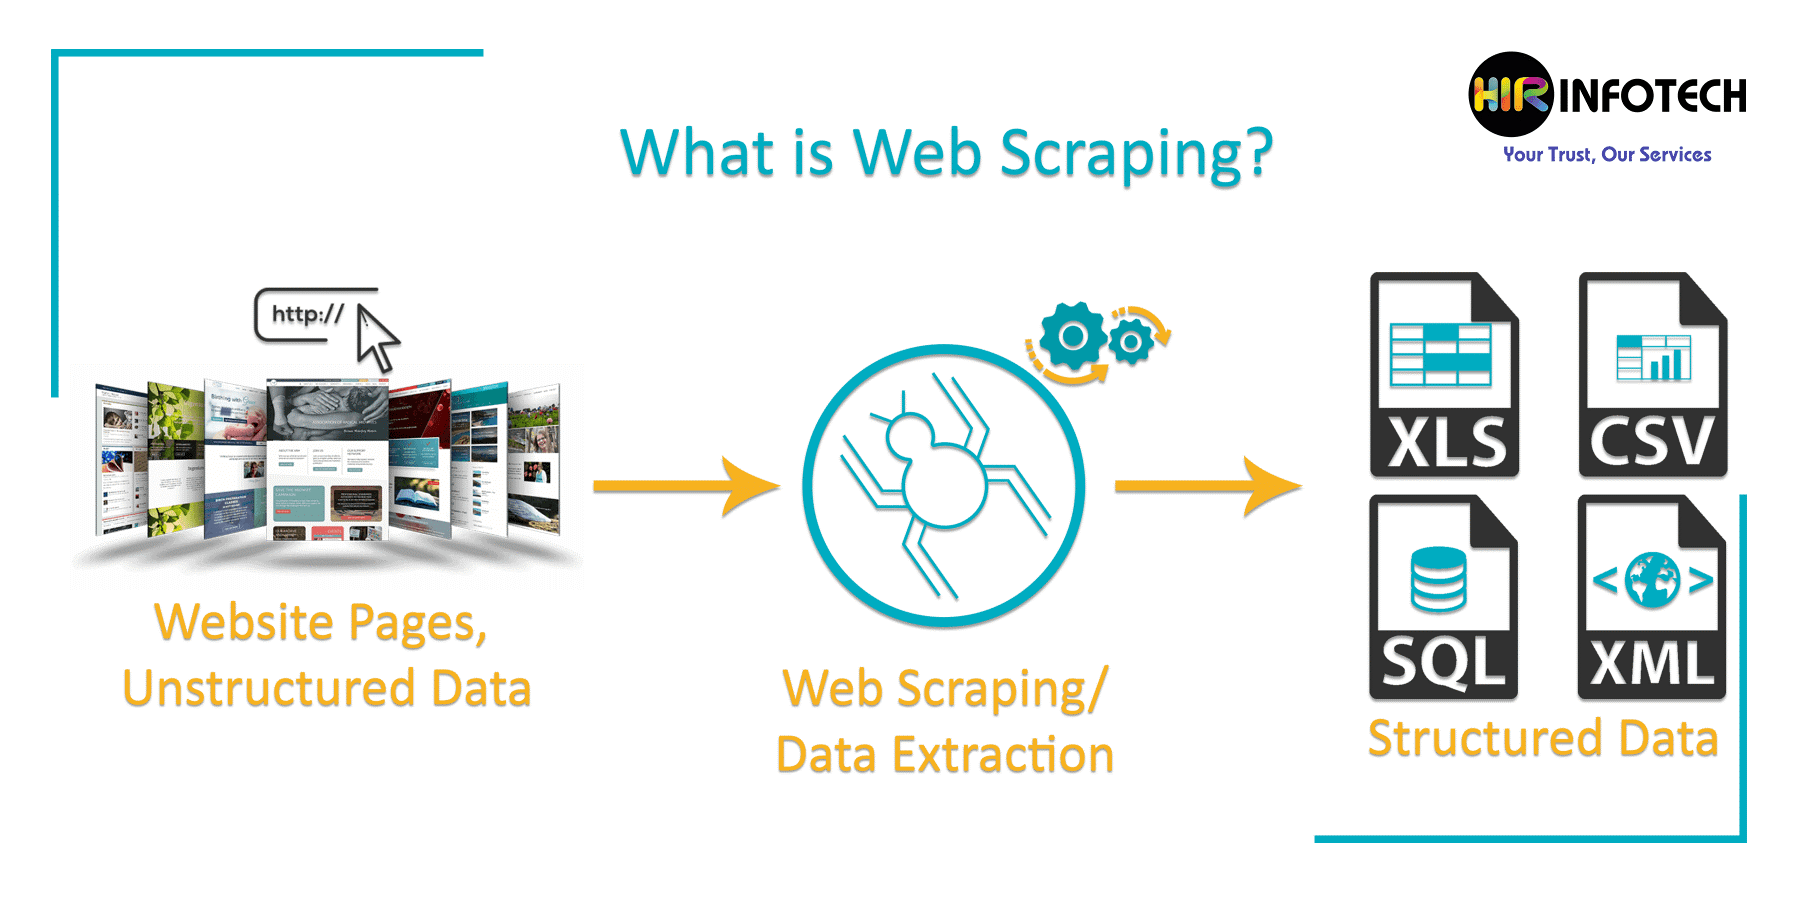
\includegraphics[width=8cm, height=4cm]{img/scraping.png}
							\end{figure}
						
						\item \textbf{ Extracción de datos con Python}
						
							En este ejemplo con librerías como BeautifulShop que nos sirve para la extracción sencilla de datos concretos de una página web en HTML sin excesiva programación. Es lo que técnicamente recibe el nombre de parsear HTML. Una de las ventajas de esta biblioteca en Python es que todos los documentos salientes de la extracción de datos lo hacen en UTF-8, lo cual es bastante interesante porque el problema típico de las codificaciones queda totalmente resuelto
							Document Parsing (Análisis de documentos):\\

							Se utiliza para analizar diferentes tipos de documentos como pdf, html, doc, presentaciones o imágenes. En algún momento es necesario que conserve el formato y la disposición del documento original, por ejemplo, en ocasiones, las estructuras originales de los párrafos, las estructuras de las tablas, los encabezados y subtítulos y el mapeo de las secciones respectivas son importantes para una mejor precisión, por lo que debe conservarlos.\\
							
							
							
						\item \textbf{ Tokenización}
						
							Se trata de dividir el texto en varias oraciones, ya que ciertos procesos solo toman una oración por vez. De manera similar, las oraciones deben convertirse en una secuencia de fichas para ciertos pasos.\\
						
						Aplicaciones de Datos no estructurados. \\
						
						\begin{itemize}
							
							\item \textbf{  Habla } \\
								
								Modelando la relación entre audio y palabras dichas se
								pueden implementar sistemas que hagan las siguientes
								tareas: \\
								 
								 \begin{itemize}
								 	
								 	\item Automatic speech recognition (nos permite pasar a análisis de texto).
								 	\item Speech synthesis. 
								 	
								 	\begin{figure}[htb]
								 		\centering 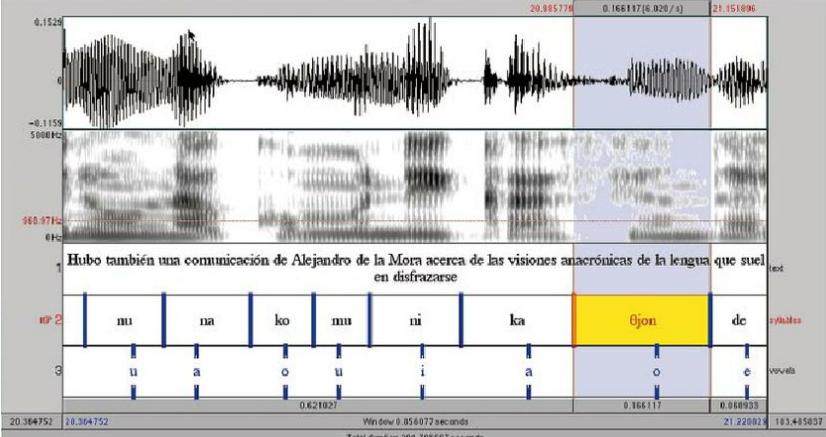
\includegraphics[width=8cm, height=4cm]{img/tokenizacion.png}
								 	\end{figure}
								 \end{itemize}
				\newpage
							\item \textbf{ Predicción de pobreza usando imágenes satelitales}\\
							
							\begin{figure}[htb]
								\centering 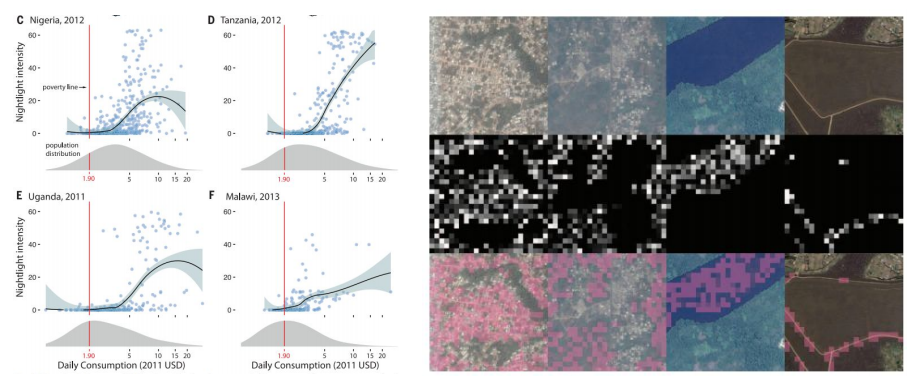
\includegraphics[width=8cm, height=4cm]{img/prediccion.png}
							\end{figure}
						
							\item \textbf{ Clasificacion de imágenes}
							 
							 \begin{figure}[htb]
							 	\centering 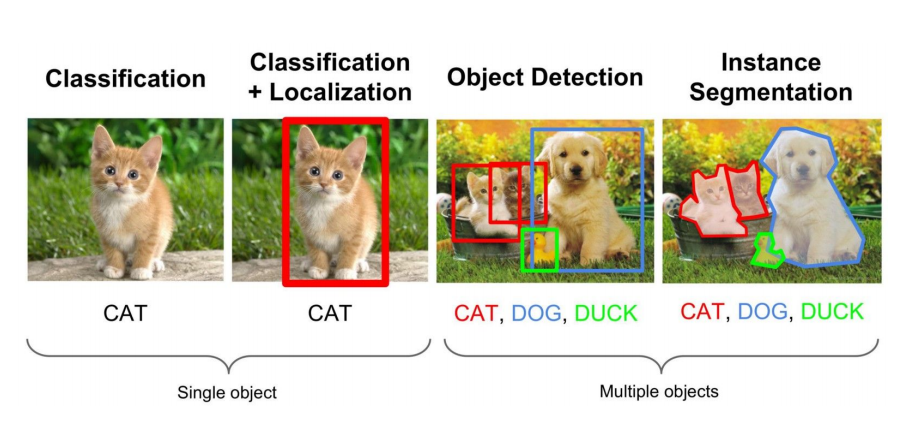
\includegraphics[width=8cm, height=4cm]{img/clasificacion.png}
							 \end{figure}
						 
							\item \textbf{ Ejemplo sencillo tratamiento datos no estructurados (redes sociales)}\\
							
								Dada la variada naturaleza de los datos no estructurados, hay infinidad de posibles procesos relacionados con ellos.  \\
								
								El objetivo de este análisis de datos es conocer la percepción que existe sobre el precio de determinado producto en twitter.\\
								
								
								\begin{itemize}
									
									\item \textbf{Extracción:}  Utilizando una clase de java (ejemplo twitter4j) leemos el feed de Twitter disponible en https://twitter.com/search/realtime. Añadimos a los campos disponibles calificaciones del tipo: idioma, localización geográfica.
									
									\item \textbf{ Transformación:} Filtramos todos aquellos tuits que contengan el nombre del producto. Refinamos el filtro introduciendo campos del tipo (“precio” ) +  (“barato”, “caro”, “económico”, etc..) , teniendo en cuenta el idioma en el que  se generan lo tuits. Valorar la opción en base al volumen de obtener una muestra representativa de los datos extraídos y filtrados.
									
									\item \textbf{  Volcado a BBDD :} Insertamos en una tabla el registro del tuit con la calificación identificada (idioma, localización geográfica).
									
									\item \textbf{ Informes:} Creamos informe que permita realizar análisis por tiempo y campos de calificación. Hay que considerar que este informe puede ser actualizado en tiempo real.
									
									
									
									
								\end{itemize}
							
							
						\end{itemize}
						
						
						
					\end{enumerate}
				
				
					
				\end{enumerate}
		\item \textbf{Conclusiones } 
		
		 \begin{itemize}
			

			\item Concluimos que no sólo los datos estructurados pueden ser analizados y que existen muchos más tipos de datos.
			
			\item Hay una gran disponibilidad de datos no estructurados.
			
			\item Actualmente existen múltiples técnicas para analizar distintos tipos de datos no estructurados.
			
			\item En la actualidad, todo lo que tenga que ver con los Datos no estructurados está creciendo exponencialmente.
			
			
		\end{itemize}
	
		\item \textbf{Bibliografia } 
				
			\begin{itemize}
			
			 
			\item Datos no Estructurados. 
			Recuperado de: https://sommet.mx/blog/que-son-los-datos-no-estructurados
			
			 \item Diferencia entre datos estructurados y no estructurados. Recueperado de: https://www.kyoceradocumentsolutions.es/es/smarter-workspaces/insights-hub/articles/diferencia-entre-datos-estructurados-y-no-estructurados.html#:~:text=Los\%20datos\%20no\%20estructurados\%2C\%20generalmente,y\%20almacenan\%20de\%20manera\%20organizada.
			
			\item Herramientras de extracción de datos. 
			Recuperado de: https://bbvaopen4u.com/es/actualidad/herramientas-de-extraccion-de-datos-para-principiantes-y-profesionales
			
			\item Extraccion y analizis de datos no estructurados.
			Recuperado de: http://www.eco.unc.edu.ar/files/ief/workshops/2018/Galvez_Extraccin_y_Anlisis_de_Datos_No_Estructurados__Aplicaciones_usando_texto_audio_imgenes_y_video.pdf
			
			
			
			
		\end{itemize}
		
		
		
	\end{enumerate}
	
	

\end{document}
